%% ITEM 0 TYPE Section
\section{Methods (your approach)}%% ITEM 1 TYPE Section
%% ITEM 1 TYPE Section
\section{Methods: CSPG Approach}%% ITEM 2 TYPE Frame
%% ITEM 2 TYPE Frame
\begin{frame}
\frametitle{CSPG: Core Idea}

\begin{columns}
\begin{column}{0.5\textwidth}
\begin{itemize}
\item \textbf{Random partitioning} of dataset $\mathcal{D}$ into groups
\item Each group shares \textbf{routing vectors} (red)
\item Build \textbf{sparser, smaller graphs} for each partition
\item $\mathcal{G}_1$ (left) and $\mathcal{G}_2$ (right) in example
\end{itemize}
\end{column}
\begin{column}{0.5\textwidth}
\begin{figure}
\centering
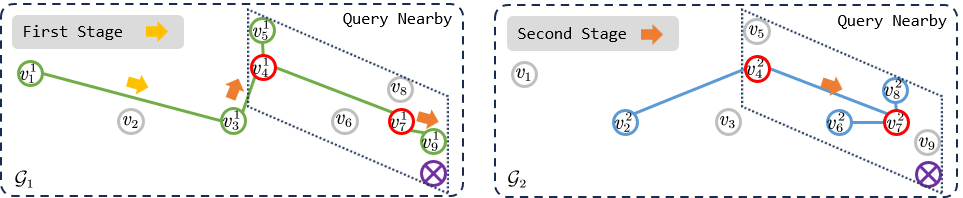
\includegraphics[width=0.9\textwidth,height=0.7\textheight,keepaspectratio]{picture/method.png}
\caption{Partitioning strategy with routing vectors}
\end{figure}
\end{column}
\end{columns}

\vspace{5mm}
\textbf{Key Benefits:}
\begin{itemize}
\item Sparse graphs allow \textbf{larger steps} for fast approach
\item Routing vectors enable \textbf{cross-partition navigation}
\item Two-stage search: \textbf{fast approaching + precise search}
\end{itemize}
\end{frame}%% ITEM 3 TYPE Frame
%% ITEM 3 TYPE Frame
\begin{frame}
\frametitle{Two-Stage Search Algorithm}

\textbf{Stage 1: Fast Approaching}
\begin{itemize}
\item Start from routing vectors in \textbf{one partition}
\item Navigate sparse graph $\mathcal{G}_i$ toward query $q$
\item Stop when distance stops decreasing significantly
\item \textbf{Output}: candidate set $\mathcal{C}_i$ from partition $i$
\end{itemize}

\vspace{5mm}
\textbf{Stage 2: Precise Search}
\begin{itemize}
\item For each candidate $c \in \mathcal{C}_i$, examine its \textbf{routing neighbors}
\item These neighbors belong to \textbf{other partitions}
\item Expand search across partitions using routing connections
\item \textbf{Final result}: nearest neighbors from entire dataset
\end{itemize}

\vspace{5mm}
\textbf{Algorithm Complexity:}
\begin{itemize}
\item Stage 1: $O(\log n)$ distance computations
\item Stage 2: $O(k \cdot m)$ where $k$ is candidate size, $m$ is routing degree
\item \textbf{Total}: Much fewer than exhaustive search
\end{itemize}
\end{frame}%% ITEM 4 TYPE Frame
%% ITEM 4 TYPE Frame
\begin{frame}
\frametitle{Summary: CSPG Advantages}

\begin{itemize}
\item \textbf{Efficiency}: Sparse graphs reduce distance computations
\item \textbf{Scalability}: Partitioning enables parallel processing
\item \textbf{Accuracy}: Cross-partition expansion ensures high recall
\item \textbf{Flexibility}: Works with various graph construction methods
\end{itemize}

\vspace{5mm}
\textbf{Key Innovations:}
\begin{itemize}
\item Random partitioning with shared routing vectors
\item Two-stage search: fast approaching + precise expansion
\item Sparse graphs for large-step navigation
\item Cross-partition connectivity via routing neighbors
\end{itemize}

\vspace{5mm}
\textbf{Next}: We'll evaluate CSPG against state-of-the-art methods on benchmark datasets.
\end{frame}%% ITEM 5 TYPE Section
%% ITEM 5 TYPE Section
\section{Conclusion (contributions)}%% ITEM 6 TYPE Frame
%% ITEM 6 TYPE Frame
\begin{frame}
\frametitle{Conclusion: Key Contributions of CSPG}

\begin{itemize}
    \item \textbf{Novel Partitioning Strategy}: CSPG randomly partitions datasets to create smaller, sparser proximity graphs
    \item \textbf{Efficient Two-Stage Search}: Combines fast proximity search with cross-partition precise expansion
    \item \textbf{Balanced Performance}: Achieves optimal trade-off between speed (QPS) and accuracy (Recall@10)
    \item \textbf{Practical Improvements}: Demonstrates consistent performance gains across multiple datasets and graph algorithms
\end{itemize}

\vspace{0.5cm}
\textbf{Core Innovation}: Partitioning reduces distance computations while maintaining search quality through intelligent routing vector utilization
\end{frame}%% ITEM 7 TYPE Frame
%% ITEM 7 TYPE Frame
\begin{frame}
\frametitle{Experimental Validation: Superior Performance}

\begin{figure}[ht]
	\centering
	\includegraphics[width=0.8\textwidth,height=0.6\textheight,keepaspectratio]{picture/ann-benchmark.pdf}
	\caption{QPS vs. Recall@10 on SIFT1M dataset (ANN-Benchmarks)}
\end{figure}

\begin{itemize}
    \item \textbf{CSPG achieves higher QPS \& Recall@10} than traditional proximity graphs
    \item \textbf{1.5x speedup} for Vamana and HCNNG across all datasets
    \item \textbf{Pushes Pareto frontier outward}: Better speed without sacrificing accuracy
\end{itemize}
\end{frame}%% ITEM 8 TYPE Frame
%% ITEM 8 TYPE Frame
\begin{frame}
\frametitle{Conclusion: CSPG Achieves Superior Performance}

\begin{columns}
\begin{column}{0.5\textwidth}
\textbf{Key Contributions:}
\begin{itemize}
    \item Novel partitioning strategy creates smaller, sparser graphs
    \item Efficient two-stage search: fast proximity + cross-partition expansion
    \item Balances speed (QPS) and accuracy (Recall@10)
\end{itemize}

\vspace{0.3cm}
\textbf{Experimental Results:}
\begin{itemize}
    \item Higher QPS \& Recall@10 than traditional proximity graphs
    \item 1.5x speedup for Vamana and HCNNG
    \item Validates partitioning reduces computations while maintaining quality
\end{itemize}
\end{column}
\begin{column}{0.5\textwidth}
\begin{figure}[ht]
	\centering
	\includegraphics[width=0.95\textwidth,height=0.7\textheight,keepaspectratio]{picture/ann-benchmark.pdf}
	\caption{QPS vs. Recall@10 (SIFT1M)}
\end{figure}
\end{column}
\end{columns}
\end{frame}